\chapter{Meassurements}

\begin{figure}[H]
\centering
\begin{subfigure}[b]{0.48\textwidth}
                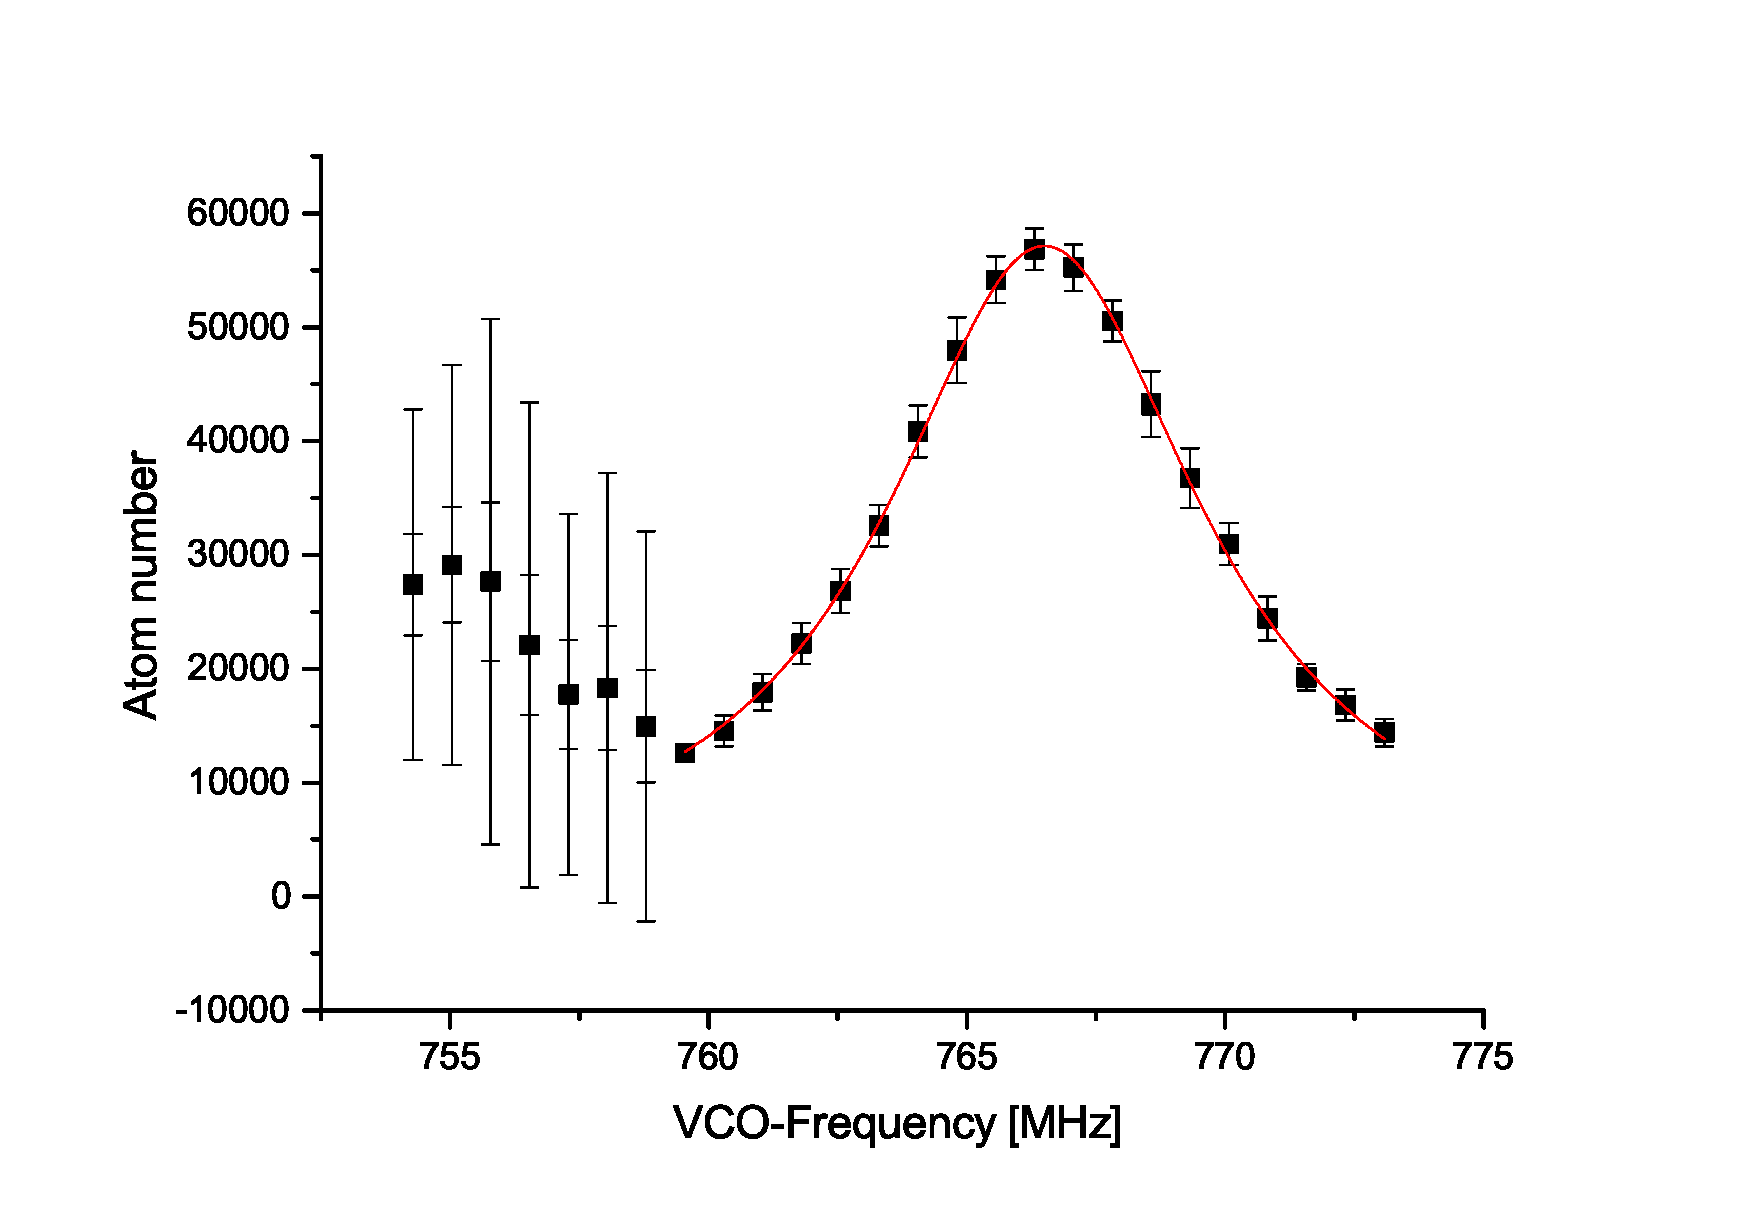
\includegraphics[width=\textwidth]{withoutodt}
                \caption{Dipole-trap turned off.}
\end{subfigure}
\begin{subfigure}[b]{0.48\textwidth}
               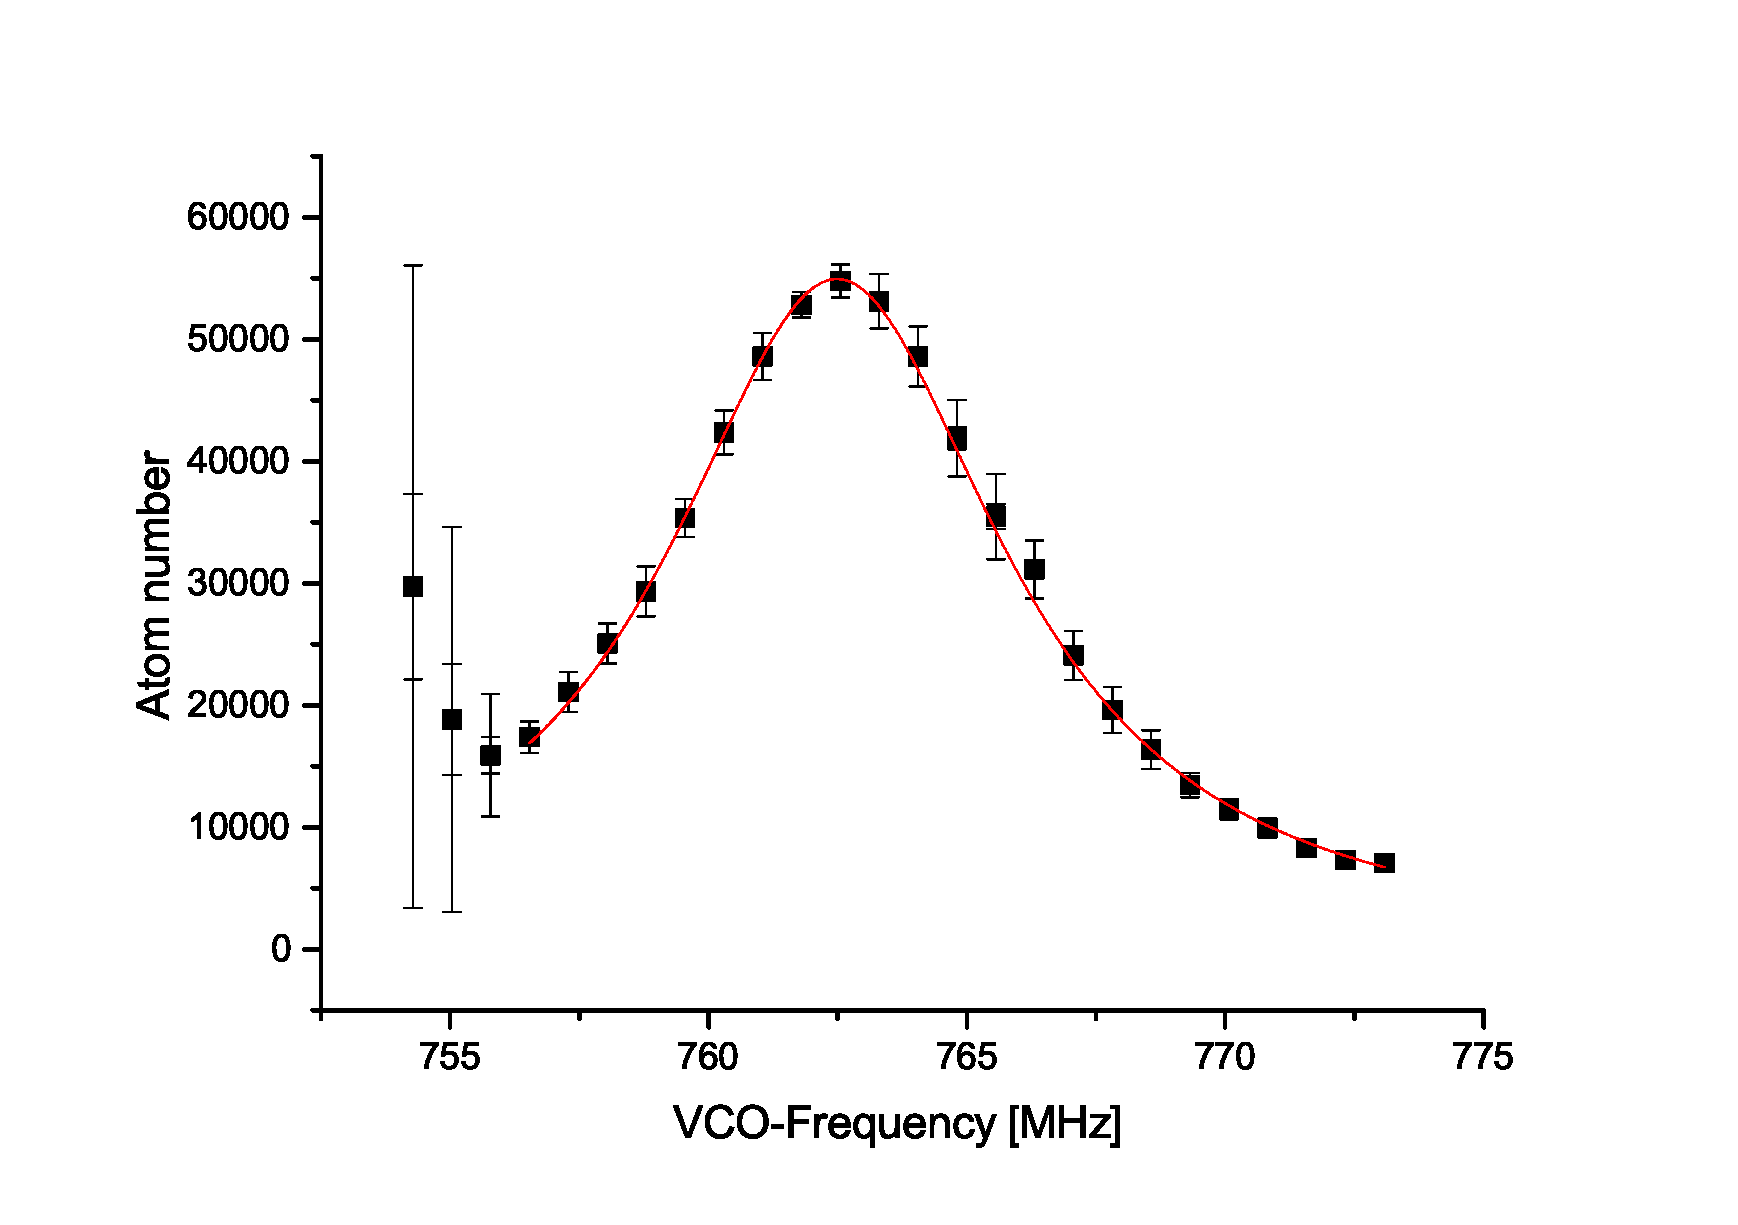
\includegraphics[width=\textwidth]{withodt}
                \caption{Dipole-trap turned on.}
\end{subfigure}


\caption{Resonance peak for the transition: $2s\rightarrow2p_{3/2}, |m_j|=3/2$ at 1070 nm.}
\label{resonance}
\end{figure}



\section{Using the meassurement to calculate trap depth}

The trap depth is a parameter, that is not easy to meassure exactly but can be a quantity, important to know. If the meassurement of the differential light shift through some sort of imaging is possible one can use this to estimate the overall depth of the trap for the respective ground and excited states.
\begin{align}
U_{\mathrm{g}}=&-\frac{1}{1-\alpha_{\mathrm{e}}/\alpha_{\mathrm{g}}}\cdot \Delta E_\delta\\
U_{\mathrm{e}}=&-\frac{1}{1-\alpha_{\mathrm{g}}/\alpha_{\mathrm{e}}}\cdot \Delta E_\delta
\end{align}

Also this meassurement can make it possible to find values for other quantities of the trap. The waist of the trap beam for example is usually not exactly easy to measure, in contrast to its power. In a large dipole-trap, as we will see, the light shift is not very complicated to meassure with a good precision. Therefore this can be used to for example calculate the waist.
\begin{align}
I=&\frac{2\epsilon_0 c}{\alpha}\cdot \Delta E_\delta\\\notag\\
w_0=&\sqrt{\frac{2P}{\pi I}}
\end{align}
In this calculation $I$ is the actual maximum-intensity forming the potential and $P$ the initial laser-power in the trap.
\begin{figure}[H]
\centering
\begin{subfigure}[b]{0.6\textwidth}
                \includegraphics[width=\textwidth]{bachwards}
\end{subfigure}
\caption{Examples of backwards-calculation for different light shifts from left to right 2.0, 4.0 and 6.0 MHz for different combinations of power and waist of the trap beam.}
\label{backwards}
\end{figure}